\documentclass[12pt,letterpaper]{article}
\usepackage[latin1]{inputenc}
\usepackage[spanish]{babel}
\usepackage{graphicx}
\usepackage[left=2cm,right=2cm,top=2cm,bottom=2cm]{geometry}
\usepackage{graphicx} % figuras
\usepackage{subfigure} % subfiguras
\usepackage{float} % para usar [H]
\usepackage{amsmath}
\usepackage{txfonts}
\usepackage{stackrel} 
\usepackage{multirow}
\usepackage{enumerate} % enumerados
\renewcommand{\labelitemi}{$-$}
\renewcommand{\labelitemii}{$\cdot$}
\author{Cesar Samuel}
\title{Caratula}
\begin{document}



\author{Cesar Calapuja}
\title{Caratula}

\begin{titlepage}
\begin{center}
\large{UNERSIDAD PRIVADA DE TACNA}\\
\vspace*{-0.025in}
\begin{figure}[htb]
\begin{center}

\includegraphics[width=8cm]{./IMAGENES/logo}
\end{center}
\end{figure}
\vspace*{0.15in}
INGENIERIA DE SISTEMAS  \\

\vspace*{0.5in}
\begin{large}
TITULO:\\
\end{large}

\vspace*{0.1in}
\begin{Large}
\textbf{TRABAJO ENCARGADO} \\
\end{Large}

\vspace*{0.3in}
\begin{Large}
\textbf{CURSO:} \\
\end{Large}

\vspace*{0.1in}
\begin{large}
BASE DE DATOS II\\
\end{large}

\vspace*{0.3in}
\begin{Large}
\textbf{DOCENTE(ING):} \\
\end{Large}

\vspace*{0.1in}
\begin{large}
 Patrick Cuadros Quiroga\\
\end{large}

\vspace*{0.2in}
\vspace*{0.1in}
\begin{large}
Integrantes: \\
Cesar Samuel Calapuja Chullunquia \\

\end{large}
\end{center}

\end{titlepage}
\newpage
\subsection{Restricting Data Using WHERE} 
\subsubsection{Ejercicio 1: Restriccion de Datos mediante SELECT} 
descripcion general  \\
En esta practica, limitada las filas mostradas con:\\
Claususla WHERE\\
Los operadores de comparacion\\
Condiciones logicas mediante los operadores AND , OR y NOT.\\
\\
\\Tareas
\begin{enumerate}[1.]
    \item Muestre los detalles del curso para la sesion Spring

\begin{center}
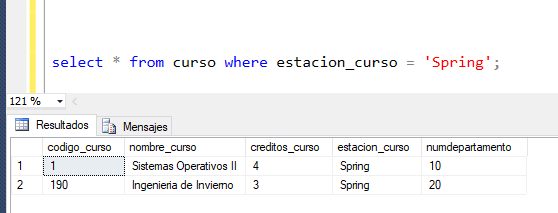
\includegraphics[width=12cm]{./IMAGENES/imagen1}
\end{center}

    
    \item Muestre los detalles de los alumnos que han conseguido una puntuacion superior a 97.
    
 
\begin{center}
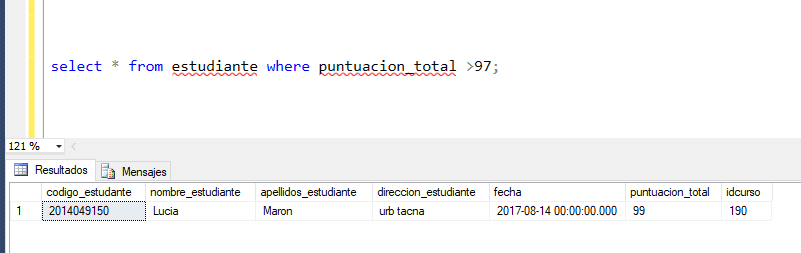
\includegraphics[width=12cm]{./IMAGENES/imagen2}
\end{center}


    \item Muestre los detalles de los alumnos que han conseguido una puntuacion entre 65 y 70.

\begin{center}
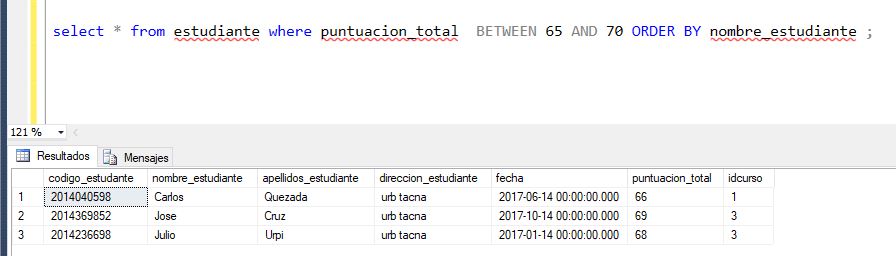
\includegraphics[width=12cm]{./IMAGENES/imagen3}
\end{center}


    
    \item Muestre a los alumnos que se registraron despues del 01-Jun-2012.
    

\begin{center}
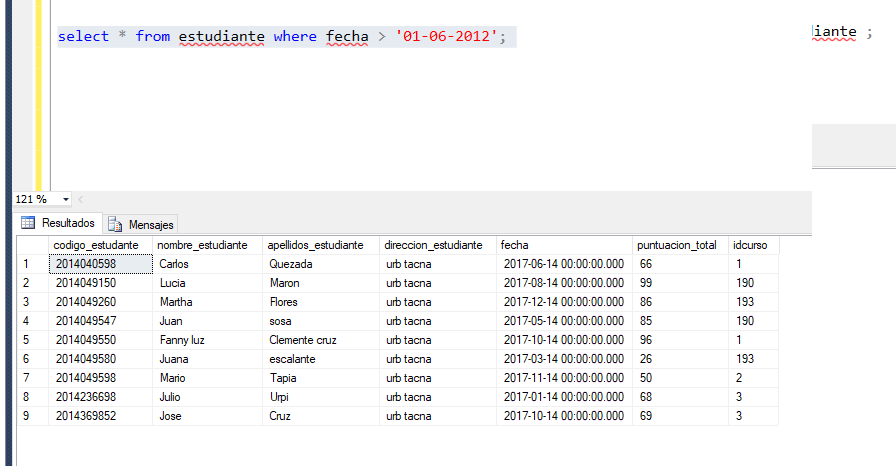
\includegraphics[width=12cm]{./IMAGENES/imagen4}
\end{center}

    \item Muestre los detalles del curso para los departamentos 10 y 30. 
    
  
\begin{center}
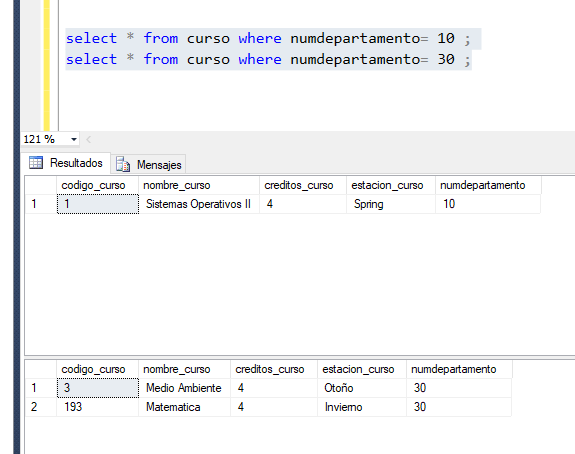
\includegraphics[width=12cm]{./IMAGENES/imagen5}
\end{center}

    \item Muestre los detalles de los alumnos cuyos nombres empiecen por la letra "J". 
  
\begin{center}
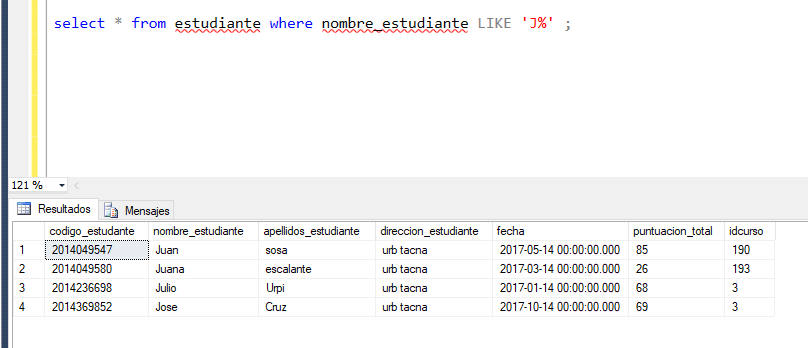
\includegraphics[width=12cm]{./IMAGENES/imagen6}
\end{center}



    \item Muestre los detalles de los alumnos que han optado por los cursos 190 o 193.

\begin{center}
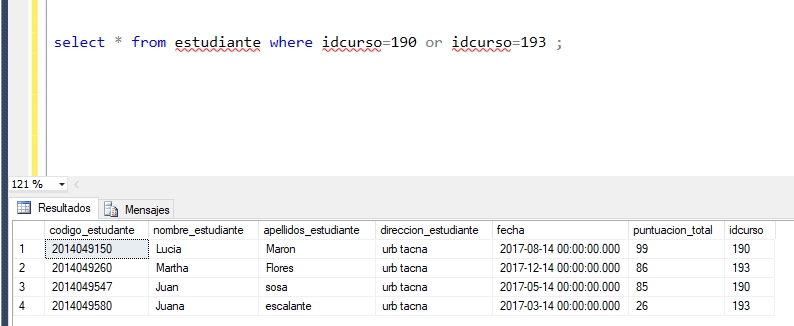
\includegraphics[width=12cm]{./IMAGENES/imagen7}
\end{center}

    \item Muestre los detalles del curso ofrecidos por el departamento 30 para la sesion de otono (identificador de sesion 200).
    

\begin{center}
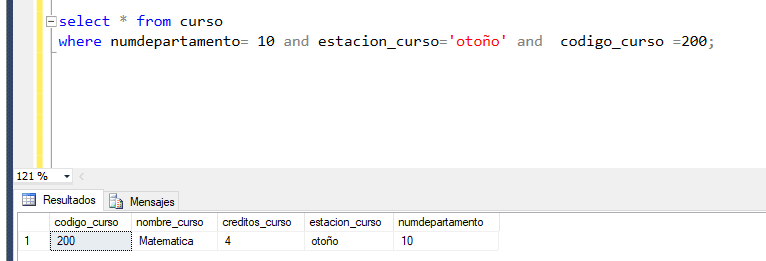
\includegraphics[width=12cm]{./IMAGENES/imagen8}
\end{center}

    
    \item  Muestre los detalles de los cursos no ofertados en la sesion de verano y otono (identificador de sesion 200 y 300).
    
 
\begin{center}
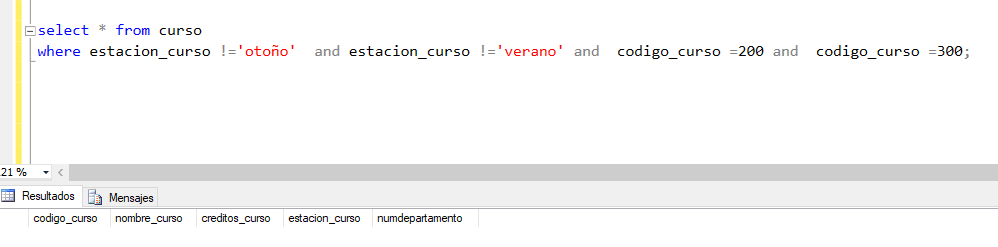
\includegraphics[width=12cm]{./IMAGENES/imagen9}
\end{center}

    \item Muestre los detalles del curso para el departamento 20.

\begin{center}
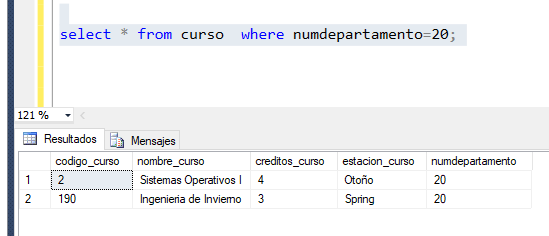
\includegraphics[width=12cm]{./IMAGENES/imagen10}
\end{center}


   
\end{enumerate}

\end{document}
